\section{Random Oracle Model}

We looked at RSA-FDH in the last section, and in this section we'll continue on and provide some semblance of a security analysis of the scheme.

As a note, collision resistance of the hash function isn't quite enough for the security of the RSA-FDH scheme. In particular, if we can find three messages $m_1, m_2, m_3$ such that $H(m_1) \cdot H(m_2) = H(m_3) \pmod{N}$ (this isn't protected against with collision resistance), then we can break the scheme, assuming that we use the RSA trapdoor function. Here, we'd have
\begin{align*}
    <<<<<<< HEAD
    \sigma_1 \sigma_2 & = f^{-1}(H(m_1)) \cdot f^{-1}(H(m_2)) \\
                      & = H(m_1)^d H(m_2)^d \pmod{N}          \\
                      & = (H(m_1) H(m_2))^d \pmod{N}          \\
                      & = H(m_3)^d \pmod{N}
    =======
    \sigma_1 \sigma_2 & = f^{-1}(H(m_1)) \cdot f^{-1}(H(m_2)) \\
                      & = H(m_1)^d H(m_2)^d \pmod{N}          \\
                      & = (H(m_1) H(m_2))^d \pmod{N}          \\
                      & = H(m_3)^d \pmod{N}
    >>>>>>> 6918b01 (added lec 11)
\end{align*}
Ideally, we'd like to have a proof of the security of this scheme, but nobody has been able to come up with one yet. Instead, we can only hope to find some kind of \emph{evidence} for the security of the scheme.

This evidence comes from the \emph{random oracle model} (ROM), otherwise known as the \emph{random oracle methodology}.

Suppose we're given a scheme $\Pi^H = (A^H, B^H, C^H, \ldots)$, where calls to the hash function $H$ is explicit. (Some functions may not call the hash function, but that's okay.)

We'd like to perform some analysis on these schemes, even though we may not fully understand the properties of the hash function---we'd like to abstract it out. To do this, we instead prove the security of $\Pi^O = (A^O, B^O, C^O, \ldots)$, where the hash function is replaced with an oracle $O$ for a truly random function.

This oracle assumption is a very strong one, and is perhaps not the most indicative of the security of the original scheme---there are cases where the scheme $\Pi^O$ under an oracle $O$ is secure, but replacing the oracle with \emph{any} instantiation breaks the security of the scheme.

When we're trying to prove security of $\Pi^O$, we'll look at an adversary $\mathcal{A}^O$, which has access to $O$. Here, observe that we can provide the answers to the oracle queries---we just need to find a contradiction to the existence of the function $\mathcal{A}$, regardless of what the oracle $O$ does.

Note here that the adversary $\mathcal{A}$ in this case is forced to explicitly call the oracle for its hash function queries---the fact that we can see these calls is called \emph{observability}. In the standard model, we can't actually see the queries that the adversary makes, since it just runs the predefined hash function itself.

Another property is called \emph{programmability}: since we're working with a random oracle, the only thing that matters is that the output of the oracle looks uniformly random. This means that we can replace a uniform output $x$ of the oracle with $f(x)$, for some one-way permutation $f$. This allows us to control some secret parameter that affects the output distribution of the oracle $O$. In the standard model, we don't have programmability---we again just have a fixed hash function that we can't change after the fact.

\begin{theorem}
    RSA-FDH is EUF-CMA secure in the ROM, assuming $\{f_s\}_s$ is a secure family of trapdoor permutations.
\end{theorem}

\begin{proof}
    Suppose we have an adversary $\mathcal{A}$ in this model.

    The first thing it is given is a public key $\mathrm{pk} = s$. The adversary then gets to make signature queries: $m \mapsto f_t^{-1}(O(m))$. At the very end, it must output a forged signature $(m^*, \sigma^*)$. This adversary is also allowed to make separate hash queries to the random oracle: $m \mapsto O(m)$. %TODO: draw the oracle calls at the top or the right side of the box

    \begin{center}
        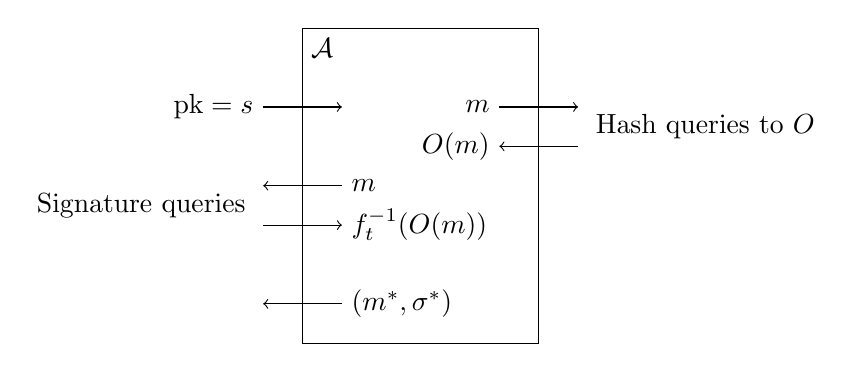
\begin{tikzpicture}
            \draw (0, 0) rectangle (3, 4);
            \node at (0.25, 3.75) {$\mathcal{A}$};

            \draw (-0.5, 3) edge[->] node[pos=0, left] {$\mathrm{pk} = s$} (0.5, 3);

            \draw (-0.5, 2) edge[<-] node[pos=1, right] {$m$} (0.5, 2);
            \draw (-0.5, 1.5) edge[->] node[pos=1, right] {$f_t^{-1}(O(m))$} (0.5, 1.5);
            \node[anchor=east] at (-0.6, 1.75) {Signature queries};

            \draw (-0.5, 0.5) edge[<-] node[pos=1, right] {$(m^*, \sigma^*)$} (0.5, 0.5);

            \draw (2.5, 3) edge[->] node[pos=0, left] {$m$} (3.5, 3);
            \draw (2.5, 2.5) edge[<-] node[pos=0, left] {$O(m)$} (3.5, 2.5);
            \node[anchor=west] at (3.6, 2.75) {Hash queries to $O$};
        \end{tikzpicture}
    \end{center}

    WLOG, suppose that for every message $m$ that $\mathcal{A}^O$ queries for a signature, it has already made a query for the same message to the hashing oracle. (Otherwise, we can simply make a wrapper around $\mathcal{A}^O$ that does this.) We can also assume WLOG that when the adversary outputs $(m^*, \sigma^*)$, it has also made the hashing query $O(m^*)$. Let's call this hybrid $H_0$.

    For the hybrid $H_1$, we'll abort the machine if for any $m, m'$ in the hash queries, we have $O(m) = O(m')$, essentially removing all collisions from the oracle. This happens with negligible probability ($q^2 / 2^n$), so this hybrid is still indistinguishable from $H_0$.

    Next, we'll construct an adversary $\mathcal{B}$ using $\mathcal{A}$, and inverts the trapdoor permutation. In particular, given $(s, y^*)$, where $y^* = f^{-1}(x^*)$, the goal is to output $x^*$.

    Suppose $\mathcal{A}$ makes $q_s$ signing queries and $q_h$ hashing queries.

    We pass in $s$ as $\mathrm{pk}$. $\mathcal{B}$ first samples an $i^* \gets \{1, \ldots, q_h\}$. We then set the output of the $i$th hash query to $y^*$. In particular, we have $O(m_{q_{i^*}}) = y^*$. If the adversary happens to call a signing query on $i^*$, we'll abort.

    We still need to specify what happens on all other queries, and we want to make sure that we can respond with a signature query on all of these other queries. For $i \ne i^*$, we sample $x \in D_s$, and compute $y = f_s(x)$. On the $i$th hashing query, we then set $O(m_i) = y$. If the adversary later requests a signature on the same $m_i$, then we output $x$ for the signing query. (This is because $f^{-1}(O(m_i)) = f^{-1}(y) = x$.)

    In particular, the adversary must have called the hashing query for its output $m^*$, and with some probability, this is the $i^*$th query, in which case the message $m^*$ is our inverse $x^*$.

    Analyzing the probabilities, we have that
    \begin{align*}
        \Pr(\text{$\mathcal{B}$ outputs $f^{-1}(x^*)$})
         & = \Pr(\text{$\mathcal{A}$ successful} \land \text{no sign query on $m_{i^*}$} \land m^* = m_{q_i^*}) \\
         & = \varepsilon \times \left(1 - \frac{1}{q_h}\right)^{q_s} \times \frac{1}{q_h}                       \\
         & \approx \frac{\varepsilon}{q_h}
    \end{align*}
    which is non-negligible, assuming $\mathcal{A}$ is successful with non-negligible probability.
\end{proof}

We'll now talk about a different scheme and analyze its security under the random oracle model.

This scheme is called the \emph{Schnorr signature scheme}. Given a group $G$ of prime order $q$ and a hash function $H : \{0, 1\}^* \to \mathbb{Z}_q$, we define
\begin{itemize}
    \item $\textsc{Gen}(1^n) = (\mathrm{pk} = g^x, \mathrm{sk} = x \gets \mathbb{Z}_q)$
    \item $\textsc{Sign}(\mathrm{sk}, m)$:
          \begin{algorithmic}
              \State $k \gets \mathbb{Z}_q$
              \State $r = g^k$
              \State $h = H(m \concat r)$
              \State $s = k + hx$
              \State $\sigma = (h, s)$
          \end{algorithmic}

    \item $\textsc{Verify}(\mathrm{pk}, m, \sigma)$:
          \begin{algorithmic}
              \State output $h \overset{?}{=} H(m \concat \frac{g^s}{\mathrm{pk}^h})$
          \end{algorithmic}
\end{itemize}

\begin{theorem}
    The Schnorr signature scheme is EUF-CMA secure in the ROM, assuming the discrete log problem is hard.
\end{theorem}

\begin{proof}
    The adversary $\mathcal{A}^O$ gets a public key $\mathrm{pk} = g^x$, can make signing queries $m \mapsto \textsc{Sign}(x, m)$ and hashing queries $(m, z) \mapsto O(m \concat z)$, for $z \in G$. $\mathcal{A}$ then returns a forgery $(m^*, \sigma^*)$.
    \begin{center}
        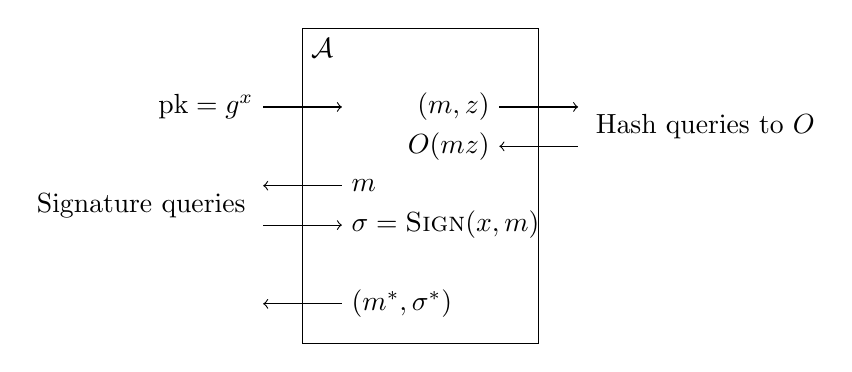
\begin{tikzpicture}
            \draw (0, 0) rectangle (3, 4);
            \node at (0.25, 3.75) {$\mathcal{A}$};

            \draw (-0.5, 3) edge[->] node[pos=0, left] {$\mathrm{pk} = g^x$} (0.5, 3);

            \draw (-0.5, 2) edge[<-] node[pos=1, right] {$m$} (0.5, 2);
            \draw (-0.5, 1.5) edge[->] node[pos=1, right] {$\sigma = \textsc{Sign}(x, m)$} (0.5, 1.5);
            \node[anchor=east] at (-0.6, 1.75) {Signature queries};

            \draw (-0.5, 0.5) edge[<-] node[pos=1, right] {$(m^*, \sigma^*)$} (0.5, 0.5);

            \draw (2.5, 3) edge[->] node[pos=0, left] {$(m, z)$} (3.5, 3);
            \draw (2.5, 2.5) edge[<-] node[pos=0, left] {$O(m \concat z)$} (3.5, 2.5);
            \node[anchor=west] at (3.6, 2.75) {Hash queries to $O$};
        \end{tikzpicture}
    \end{center}

    WLOG, we can assume that $m^* \concat r^*$ is in the list of hash queries (where $r^*$ was the value computed in the output signature $\sigma^*$).

    We'll define a modified signing algorithm as follows:
    \begin{algorithmic}
        \Function{Sign'}{$\mathrm{sk}, m$}
        \State $h, s \in \mathbb{Z}_q$ uniformly
        \State $g^k \gets \frac{g^s}{g^{hx}} = \frac{g^s}{\mathrm{pk}^h}$
        \State $h = H(m \concat g^k)$
        \State output $(h, s)$
        \EndFunction
    \end{algorithmic}
    The main idea here is to provide a random signature, consistent with the definition of $\textsc{Sign}$, so that \textsc{Verify} will still succeed.

    We'll then define a wrapper $\mathcal{A}'^{O}$, which performs these modified signing queries by itself, since it no longer requires the secret key $x$. As such, $\mathcal{A}'^O$ only makes hashing queries, and produces $(m^*, \sigma^*)$. In particular, $\mathcal{A}'$ depends on $\mathrm{pk}, q_1, h_1, \ldots, q_H, h_H$, but all of the queries $q_1, \ldots, q_H$ are deterministic depending on the previous hash output (or dependent on pk in the case of $q_1$). This means that $\mathcal{A}'$ can actually be thought of as a function of
    \[
        \mathcal{A}'(\mathrm{pk}, h_1, h_2, \ldots, h_H)
        .\]
    The main insight that we'll use is that we can run $\mathcal{A}'$ until the $(i^* - 1)$th query, and on the $i^*$th query, we run the adversary twice, on two different possible responses: $h_{i^*}$ and $h'_{i^*}$. These two executions share the first $i^* - 1$ hashing queries, and both are perfectly valid executions of the adversary. We'll use these two executions to break the discrete log problem.

    Let us define $\mathcal{B}$ that breaks the discrete log problem, given as input $(g, g^x)$. Here, we'll let $g^x$ be the public key.

    In response to hashing queries, if $\mathcal{A}'$ asks for the hash of $m \concat z$, we respond with a random value (or the same value as before if queried multiple times) as $O(m \concat z)$.

    Now, we'd like to be able to find $x$, utilizing the behavior of $\mathcal{A}'$.
    At the $i^*$th query, we run the adversary twice, with $h_{i^*}$ as the hash in the first execution, and $h'_{i^*}$ as the hash in the second execution. In the first execution, we would have gotten queries $q_{i^*}, q_{i^*+1}, \ldots, q_h$, and outputted $(m^*, \sigma^*)$. In the second execution we would have gotten queries $q_{i^*}', q_{i^*+1}', \ldots, q_h'$, and outputted $(m'^*, \sigma'^*)$.

    Now, in the $i^*$th query, note that $s = k + hx$ in the first execution, and $s' = k + h' x$ in the second execution. Crucially, the value of $k$ is the same here, since the query utilizes the same value of $r$, and we can solve for $x = \frac{s - s'}{h - h'}$.

    The probability that the adversary $\mathcal{A}'$ succeeds in producing a forgery while utilizing $i^*$ is $\mu(n) = \varepsilon(n) / q_h$. For ease, let us also define the two halves of the input to $\mathcal{A}'$ as $\alpha = (\mathrm{pk}, h_1, \ldots, h_{i^* - 1})$ and $\beta = (h_{i^*}, \ldots, h_{q_h})$. We then define the ``good set'' as
    \[
        S = \left\{\alpha \mid \Pr_{\beta}(\mathcal{A}'(\alpha, \beta)\ \text{outputs a forgery}) \ge \frac{\mu(n)}{2}\right\}
        .\]
    We can also see that $\Pr(\alpha \in S) \ge \frac{\mu(n)}{2}$; to see why, suppose by contradiction $\Pr(\alpha \in S) < \frac{\mu(n)}{2}$. Here, we have
    \begin{align*}
        \Pr(\text{$\mathcal{A}'$ succeeds}) & = \Pr(\text{$\mathcal{A}'$ succeeds} \mid \alpha \in S) \Pr(\alpha \in S) + \Pr(\text{$\mathcal{A}'$ succeeds} \mid x \notin S) \Pr(\alpha \notin S) \\
                                            & < 1 \cdot \frac{\mu(n)}{2} + \frac{\mu(n)}{2} \cdot 1 < \mu(n)
    \end{align*}
    which is a contradiction.

    The probability that $\mathcal{B}$ succeeds is thus
    \[
        \Pr(\alpha \in S) \Pr(\text{$\mathcal{A}'(\alpha, \beta)$ succeeds} \mid \alpha \in S) \Pr(\text{$\mathcal{A}'(\alpha, \beta')$ succeeds} \mid \alpha \in S)
        \ge \left(\frac{\mu(n)}{2}\right)^3
        ,\]
    due to the definition of $S$ from earlier.

    This means that in total, our probability of success is
    \[
        \Pr(\text{$\mathcal{B}$ succeeds}) \ge \frac{\varepsilon^3(n)}{8q_h^3}
        ,\]
    which is non-negligible if $\mathcal{A}'$ succeeds with non-negligible probability, giving us our contradiction.
\end{proof}
